\documentclass[]{article}
\usepackage{graphicx}
\usepackage{hyperref}
\usepackage{amsmath}
\usepackage{caption}
\usepackage{subcaption}

%opening
\title{Dynamic Light Scattering}
\author{Gunther T\"urk, Jonas Lehnen}

\begin{document}

\maketitle
\tableofcontents
\begin{abstract}
In this experiment we want to get informations about the properties of our samples by scattering light on them. Just like in nuclear physics we are able to conclude how a particle looks like by measuring the lights intensity depending on the scattering angle. Furthermore, we are interested in how long an particles movement is coherent to itself. With this information we are able to determine the Stokes radius and compare it with the radius resulting from the form factor.


Write here, what we did and learned.
\end{abstract}


\section{Theorie}
\subsection{Colloids}
Colloids are small particles, but still $10^3 to 10^4$ times larger than an atom, which are dissolved in a dispersion medium. Depending on the aggregation of state the colloidal systems are named differently. Liquid in a gaseous medium is called liquid aerosol and 2 liquids combined emulsion. Examples are mist and steam as well milk and salad dressing.
Colloids are often spherical shaped and tend to aggregate with each other. This is preventable by stabilisation techniques. The electrostatic stabilization is creatable when a colloid with groups like $~OH$ or $~SO_3H$ are dissolved in a liquid. These groups  can then dissociate as ions and the colloid becomes negative charged with a cloud of positive charged ions around it. Now the colloids are repulsing each other due to their equally charged clouds. For high salt concentrations e.g. $NaCl$ this effect is reduced. The increased amount of ions caused by the dissolved salt prevents the colloids separation of charge and with this the repulsion between colloids is reduced. 
The steric stabilisation creates this repulsive force via polymers on the colloids surface. These are preventing the aggregation by keeping them apart.

Depending particles density $n_p$ in a constant volume $V$ one can define the volume fraction $\Phi = n_p \cdot V$. This tells us about the change of phase in a colloidal system. For a system with hard spheres the crystallization form liquid starts at $\Phi=0.494$ if the increase happens in equilibrium. For a more rapid process without equilibrium the glass phase is reachable. This happens if your system freezes nearly instantaneously.  

\subsection{Light Scattering}
Considering quasi-elastic light scattering, a photon gets absorbed by the scattering center, induces a dipole moment and gets re-emitted in a different angle. The wave vector $ |\vec{k}| = \frac{2\pi n}{\lambda}$ and then the energy does not change in this assumption. Therefore the momentum change for a single photon is given by:
\begin{equation}\label{eq:momentum}
q= |\vec{k_{in}} - \vec{k_{out}}| = \frac{4\pi n}{\lambda} \cdot \sin \left( \dfrac{\Theta}{2} \right)  
\end{equation}


Using the Born approximation, we neglect every induced fields from the dipole oscillation which would again induce others molecules to oscillate. These oscillations would change our scattered light, because the  
% Born approximation erklären

	
The lasers wavelength is nearly as large as our colloids, therefore we're not allowed to use the approximation of Rayleigh scattering. By considering every colloid as its own scattering center we now can conclude how the particles are distributed in the system.

In the experiment intensity is measured. From the conclusion above we can derive a formula, just depending on the form factor $P(q)$ given by the size of the individual colloids and how they are arranged in the medium:
\begin{equation} \label{eq:intensity}
I(q) = I_0(q)b(\vec{q}=0)^2 \cdot P(q) \cdot NS(q)
\end{equation}
Where N is the number of colloids in the system and b(q) 
% was genau stellt b dar, außer komisches Ergebnis aus der Integration
\\

\begin{equation}\label{eq:form}
P(q)= \frac{9}{(qa)^6} \cdot (sin(qa) - qa \cdot cos(qa))
\end{equation}


For moving particles their dynamics are getting important. Due to Brownian motion, see \ref{hyd}, the correlation of the electric field to itself at a later time is affected. One defines the autocorrelation function 
\begin{equation}\label{eq:g1}
G_1(\vec{q}) = \langle \: \vec{E}(\vec{q},t),\vec{E}(\vec{q},t+\tau) \: \rangle
\end{equation}

Siegert relation
\begin{equation}\label{eq:siegert}
g_2(\vec{q},t) = g_1(\vec{q},t )^2 +1
\end{equation}


\subsection{Hydrodynamics}
\label{hyd}
First of all we introduce the material constant viscosity. It describes how strong the friction is for moving something through a medium. Usually it's defined as: 

%Brownian motion

\subsection{Laser and Photomultiplier}
In the experiment we are using a green $532nm$. The main principles for a laser are the inversion and the stimulated emission. Considering a 3 state energy system. Inversion is created by pumping nearly every electron from the ground state into the most excited state, this means sending in photons with the transition frequency as energy. This frequency is only for the pumping and usually higher than the lasers one. The most excited state should decay fast to the middle state that should have a long lifetime. There the electrons will wait for a photon in laser frequency to stimulate the emission of an exact identically photon. This means we end up with a electron in the ground state and two photons instead of one. Due to their same properties, i.e. same frequency and phase relation to each other, a laser creates coherent light.

The function of a photomultiplier relies on the photoelectric effect. Hereby a photon collides with a cathode and triggers an electron to leave the material.
Due to a increasing potential between the cathode and the following dynodes the electron will always hit the next potentially higher dynode. Thereby it gains more speed and is able to knock more electrons out of the dynode. Due to their shape the electrons won't skip any dynode and the amount of electrons travelling increases exponentially this the amount of dynodes. At the end they'll get absorbed from the anode to measure the current and thereby getting a signal that the cathode was hit by a photon.

\newpage
\section{Experiment}
\subsection{Setup}
The following figure shows how the basic arrangement of hardware was. Everything was controllable by the given software. Except the sample change had to be done manually. The positioning of the sample was a little bit difficult. The holder was only a small hole in a cap for the isopropyl alcohol container and the sample was placed by the friction with this hole. We tried to align it straight downwards, but it could have been tilted. The refractive index of isopropyl alcohol is $n=1.37927$ for $T=293K$. The measured temperature for the sample was $19.6 ^\circ C$ with an digital infra-red thermometer. Therefore we are using the literature value as given above.

\begin{figure}[!htbp]
\centering
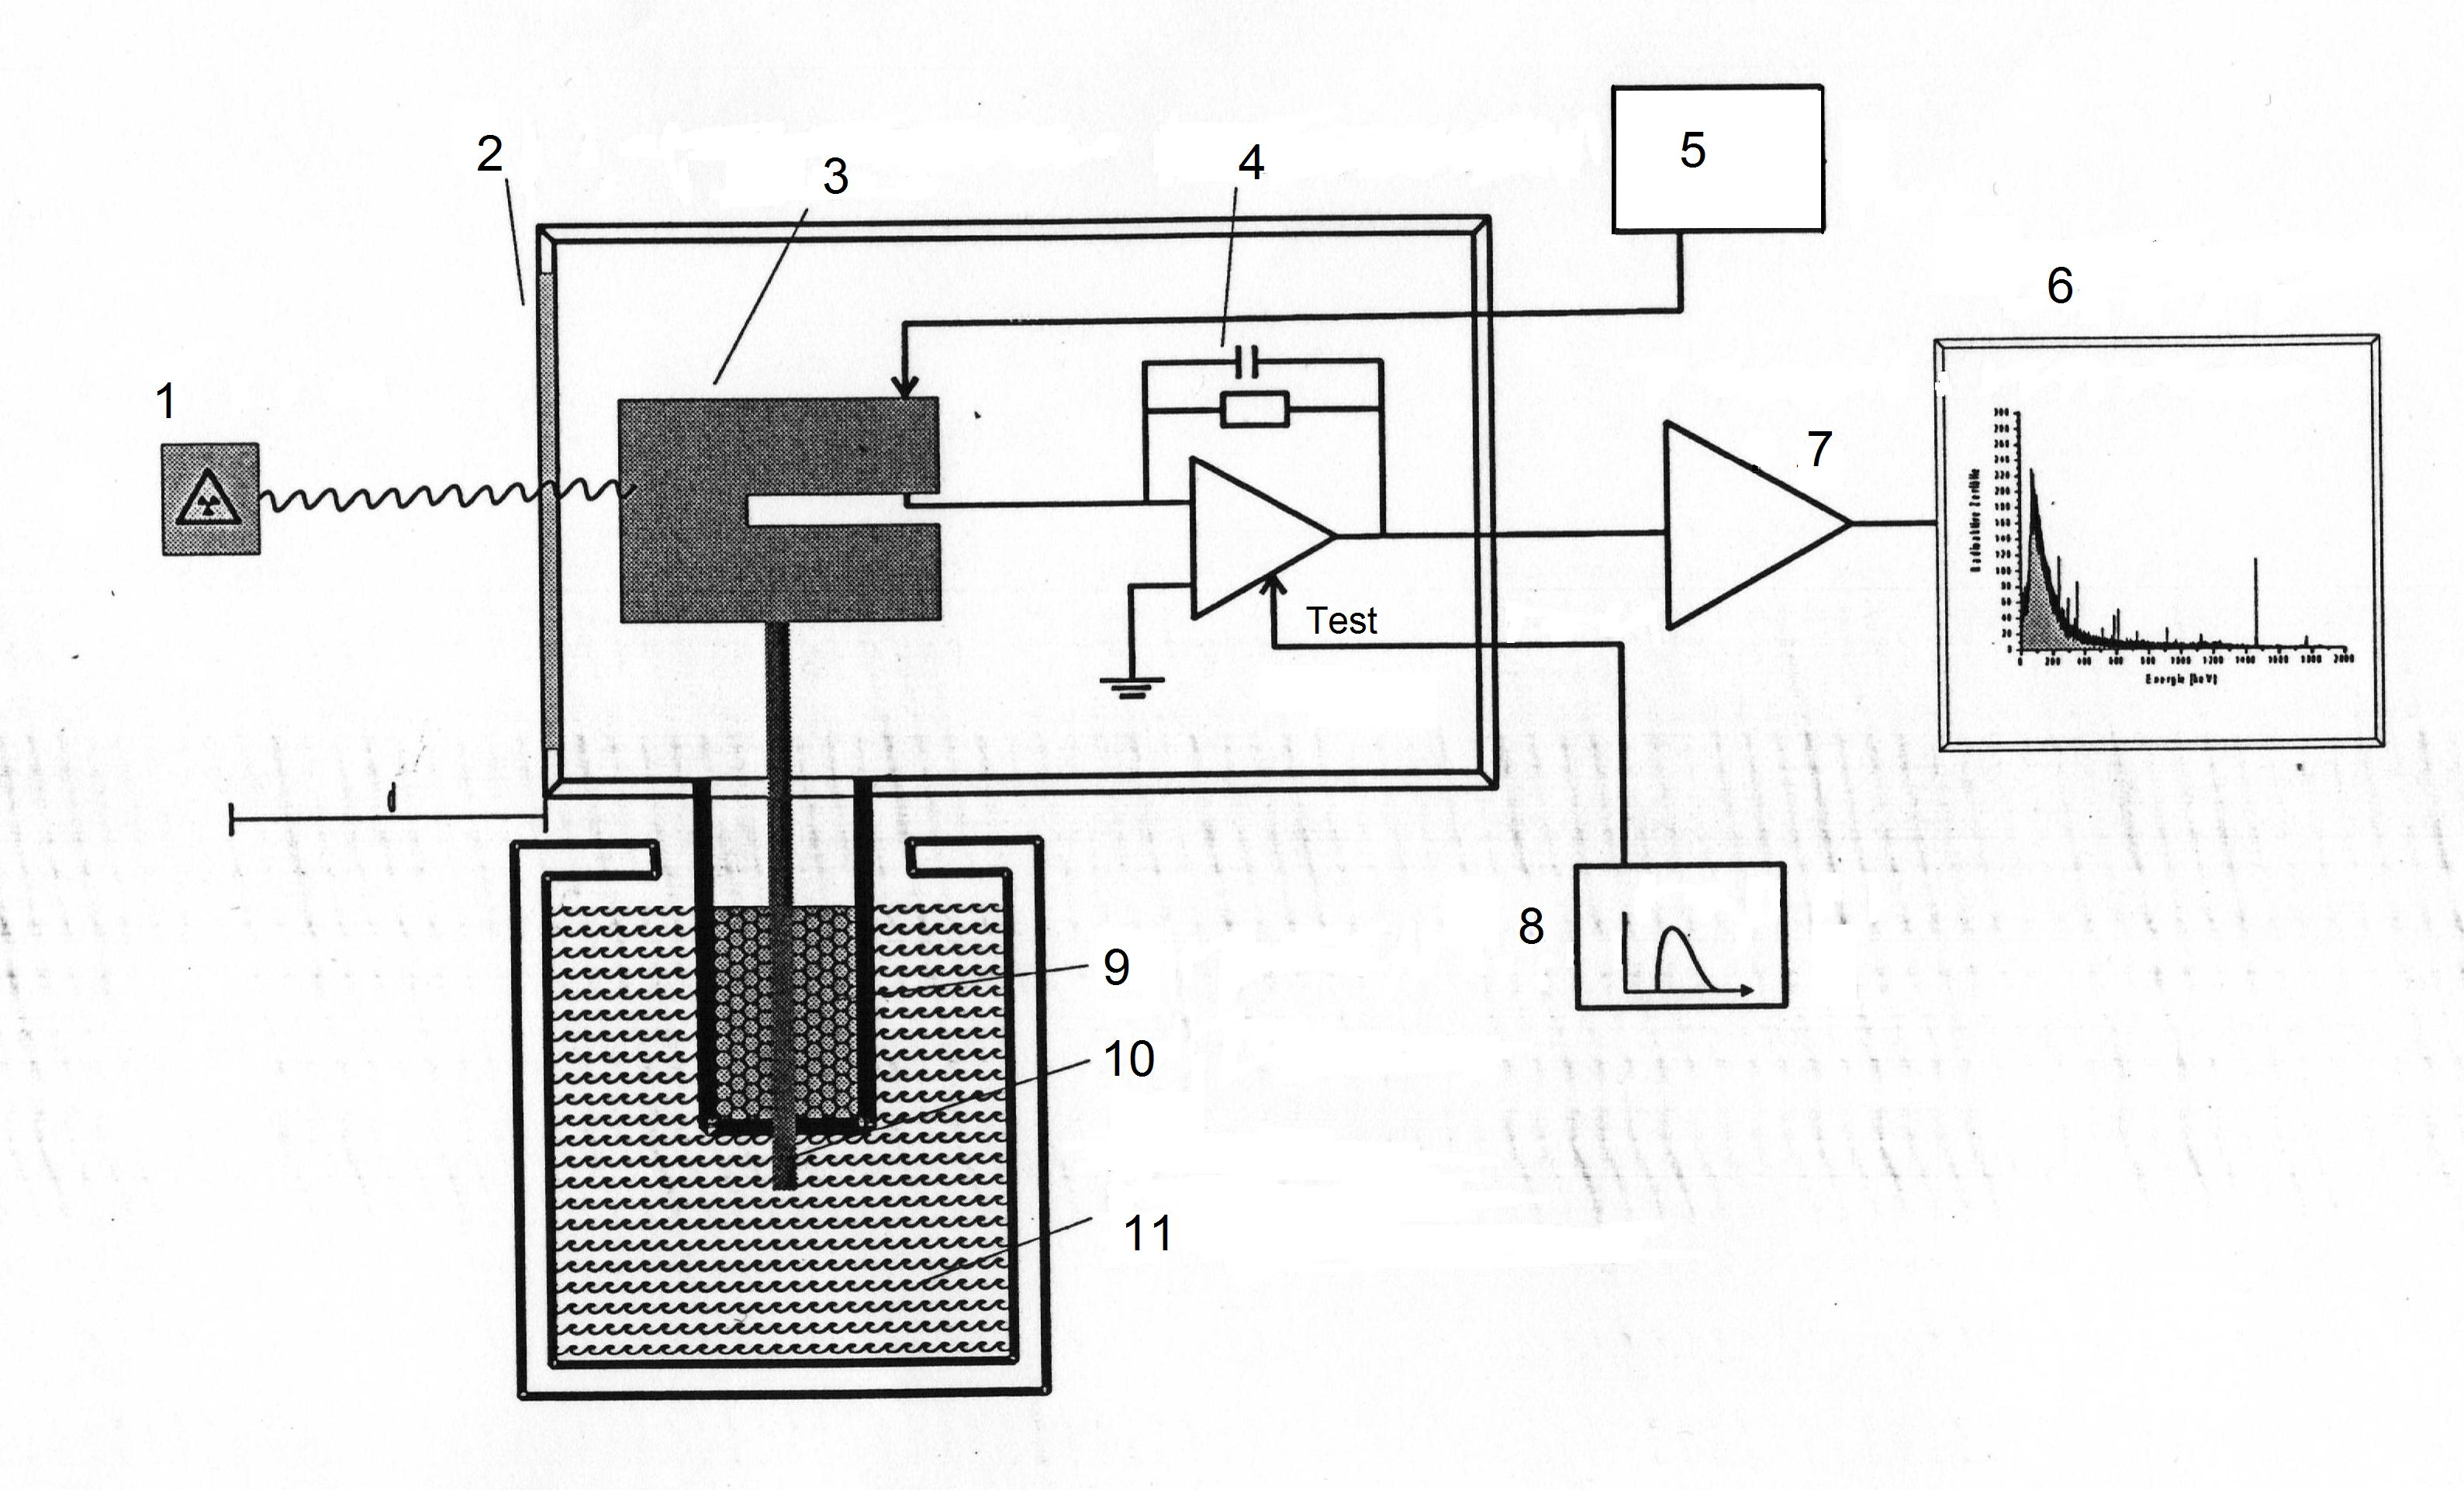
\includegraphics[width=0.8\linewidth]{Plots/Setup.png}
\caption{The experimental Set-up for our the Dynamic Light Scattering experiment. Figure taken from the given script.}
\end{figure}

We used green $532nm$ laser light for the scattering at the samples. To avoid static installations and prevent displacements in the lights path, optical fibres were used. The goniometer itself was purely adjustable by electronics to get an exact angle measurement.


\subsection{A: Small particles in fluid phase}


For fitting the form factor of the colloids we'll use equation (\ref{eq:intensity}). Thereby we introduce another constant value A in (\ref{eq:form}) which absorbs everything factor independent of q this means except of $P(q)$ and $S(q)$. The structure function is nearly 1 for very dilute samples. The assumption that there are very few colloids in the medium is justified because we couldn't see any real particles with the naked eye. 

\begin{figure}[!htbp]
\centering
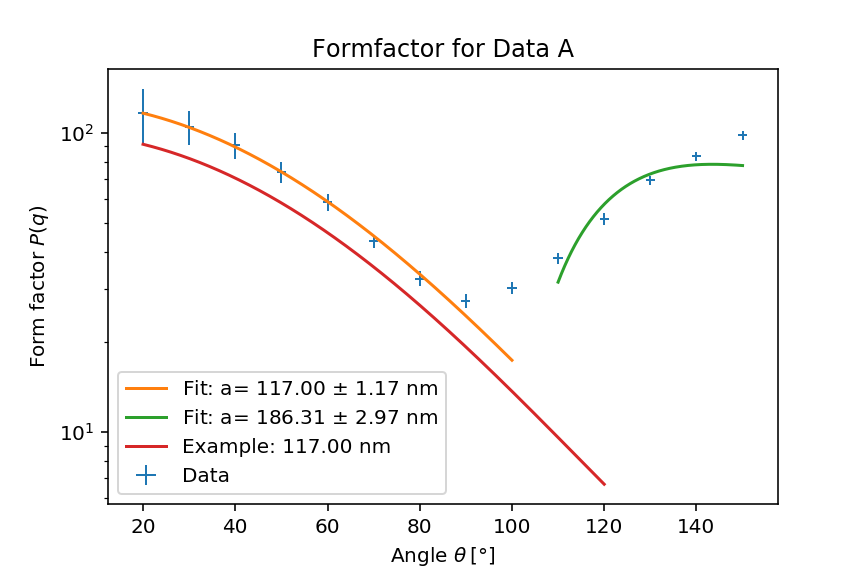
\includegraphics[width=0.8\linewidth]{Plots/FormA.png}
\caption{Intensity fitted for the form factor.}
\label{FormA}
\end{figure}

Before fitting the intensity has to be corrected. Due to the change in momentum related to the scattering angle. To get the angle independent intensity our measured mean intensities has to be multiplied by $sin(\frac{\theta}{2} )$.

% Description of the fit


\subsection{B: Large particles in fluid phase}


\subsection{C: Small particles in fluid phase, high concentration}

\begin{figure}[!htbp]
\centering
\includegraphics[width=0.8\linewidth]{Plots/"C bei 40".png}
\caption{Autocorrelation for the Sample C at 40 degrees.}
\label{C}
\end{figure}


\newpage
\subsection{D: Small particles in crystalline phase}
The last sample was clearly different from the other. One already could see a light white coloured gleam due to the high concentration which causes the crystalline phase. 

\begin{figure}[!htbp]
\centering
\includegraphics[width=0.8\linewidth]{Plots/"D bei 40".png}
\caption{Autocorrelation for the Sample D at 40 degrees. It shows a second slope which is caused by the newly formed crystalline structure in the medium.}
\label{D}
\end{figure}

As pictured in Figure \ref{D} a second slope appears for the crystalline phase. The high concentration forces the particles to come together and thereby form new structures which also causes the white gleam. These new structures are now larger than the usual particles moving in the medium. Thereby they will show a different decay time for the correlation of their momentum.


\newpage
\section{Appendix}

\subsection{Autocorrelation A}
\label{autocorr A}
\begin{figure}[!h]
\centering

\begin{subfigure}{0.48\textwidth}
\includegraphics[width=\linewidth]{Plots/A/20.png}
\end{subfigure}
\begin{subfigure}[c]{0.48\linewidth}
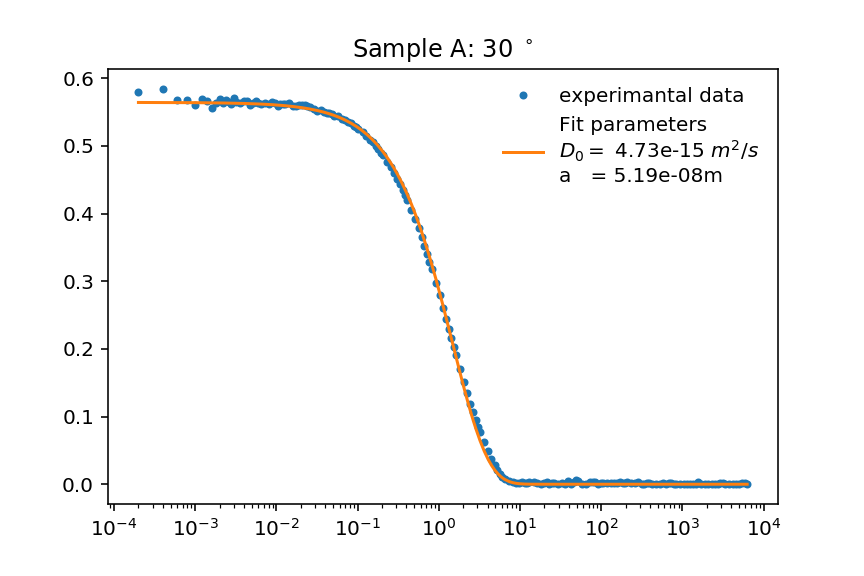
\includegraphics[width=\linewidth]{Plots/A/30.png}
\end{subfigure}

\medskip
\begin{subfigure}{0.48\textwidth}
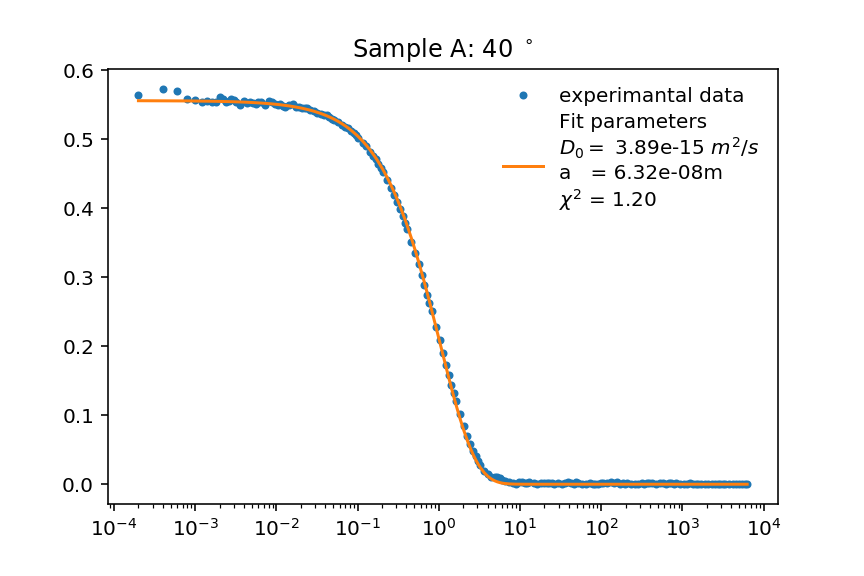
\includegraphics[width=\linewidth]{Plots/A/40.png}
\end{subfigure}
\begin{subfigure}[c]{0.48\linewidth}
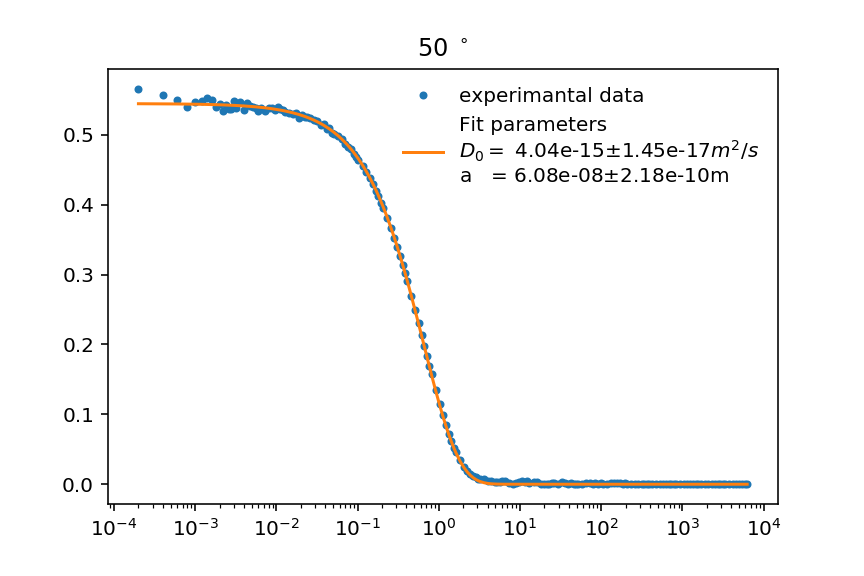
\includegraphics[width=\linewidth]{Plots/A/50.png}
\end{subfigure}

\medskip
\begin{subfigure}{0.48\textwidth}
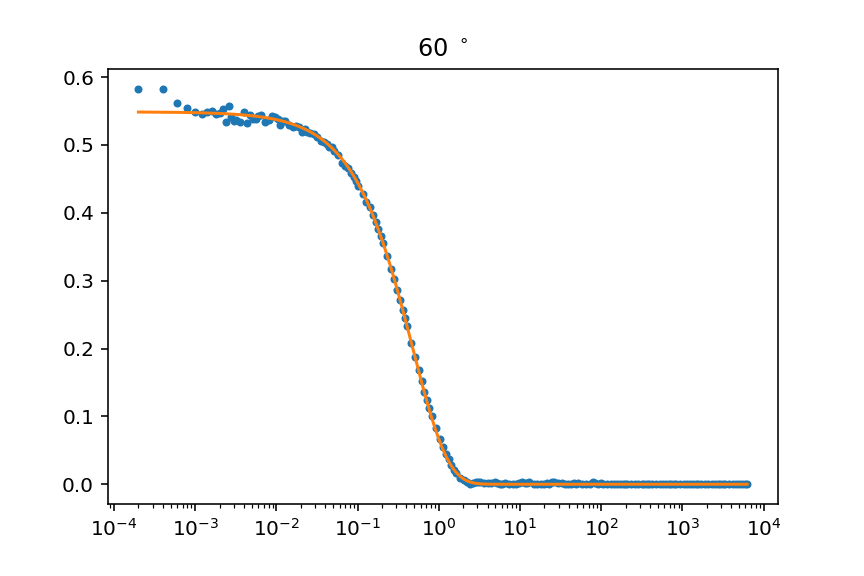
\includegraphics[width=\linewidth]{Plots/A/60.png}
\end{subfigure}
\begin{subfigure}[c]{0.48\linewidth}
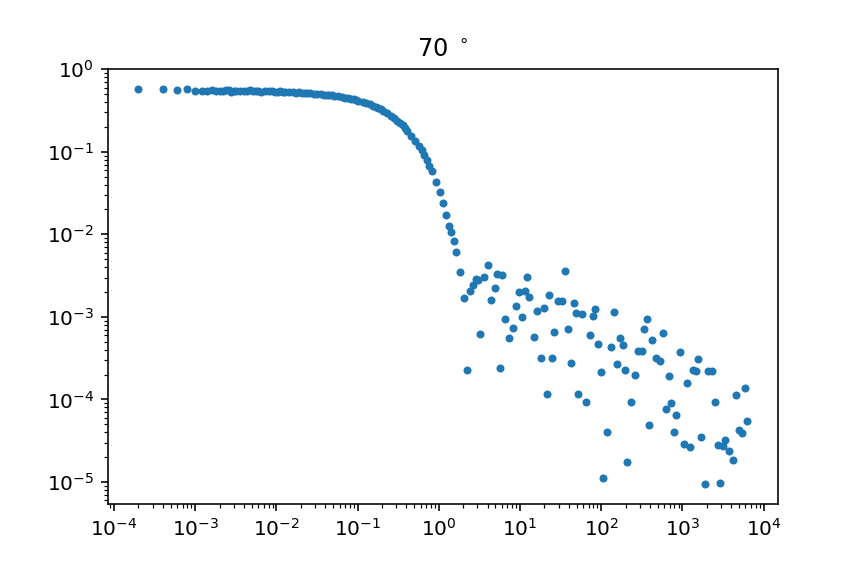
\includegraphics[width=\linewidth]{Plots/A/70.png}
\end{subfigure}

\caption{Autocorrelation Sample A: Angle between 20 and 70 degrees.}
\end{figure}
\newpage

\begin{figure}[!h]
\centering

\medskip
\begin{subfigure}{0.48\textwidth}
\includegraphics[width=\linewidth]{Plots/A/80.png}
\end{subfigure}
\begin{subfigure}[c]{0.48\linewidth}
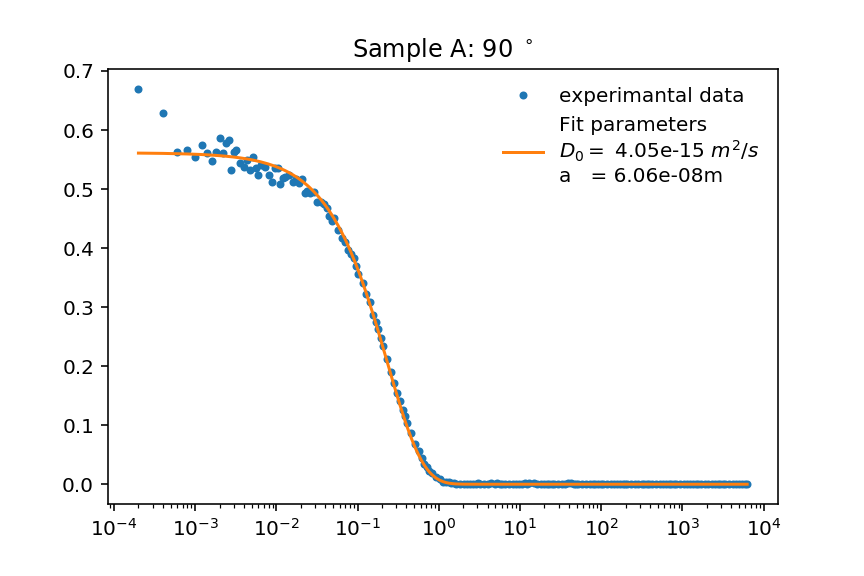
\includegraphics[width=\linewidth]{Plots/A/90.png}
\end{subfigure}

\medskip
\begin{subfigure}{0.48\textwidth}
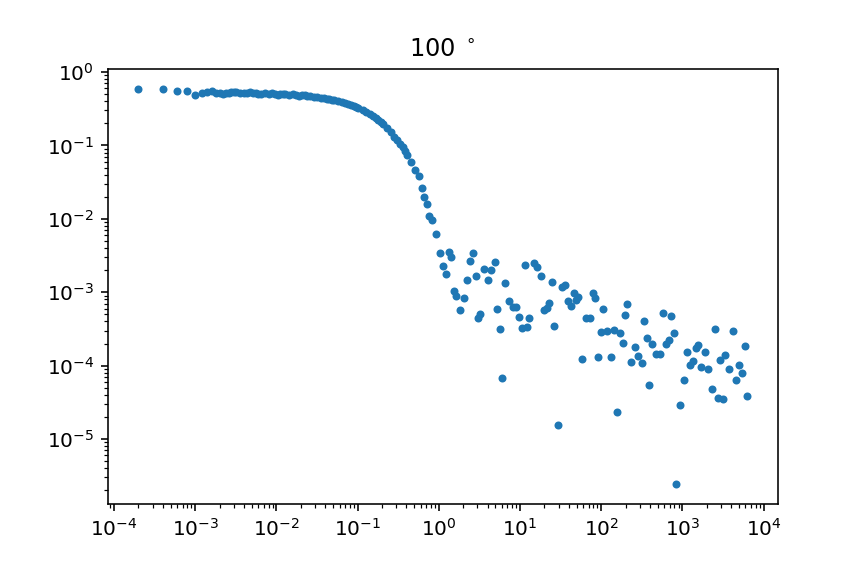
\includegraphics[width=\linewidth]{Plots/A/100.png}
\end{subfigure}
\begin{subfigure}[c]{0.48\linewidth}
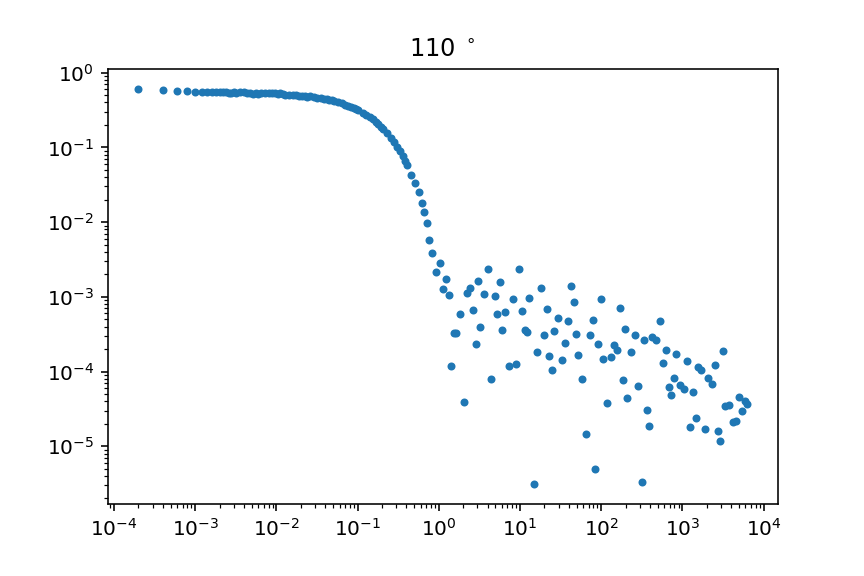
\includegraphics[width=\linewidth]{Plots/A/110.png}
\end{subfigure}

\medskip
\begin{subfigure}{0.48\textwidth}
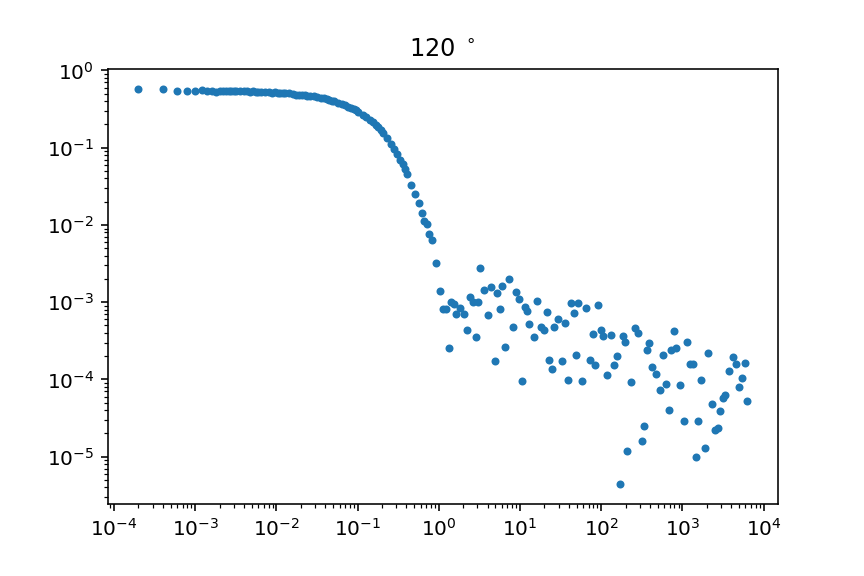
\includegraphics[width=\linewidth]{Plots/A/120.png}
\end{subfigure}
\begin{subfigure}[c]{0.48\linewidth}
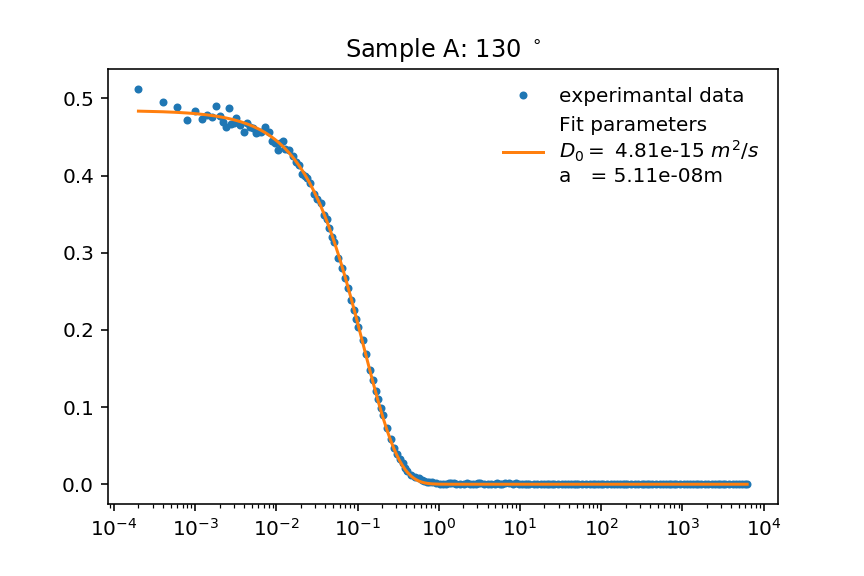
\includegraphics[width=\linewidth]{Plots/A/130.png}
\end{subfigure}

\medskip
\begin{subfigure}{0.48\textwidth}
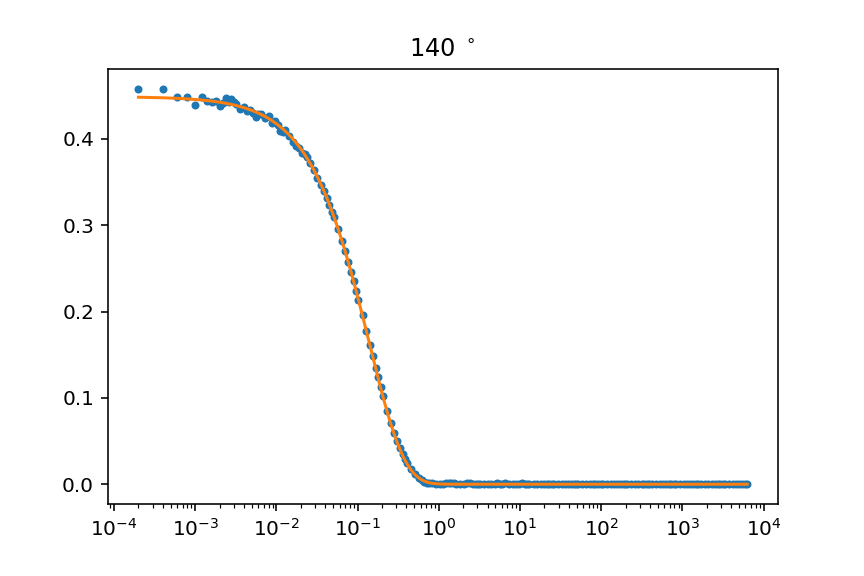
\includegraphics[width=\linewidth]{Plots/A/140.png}
\end{subfigure}
\begin{subfigure}[c]{0.48\linewidth}
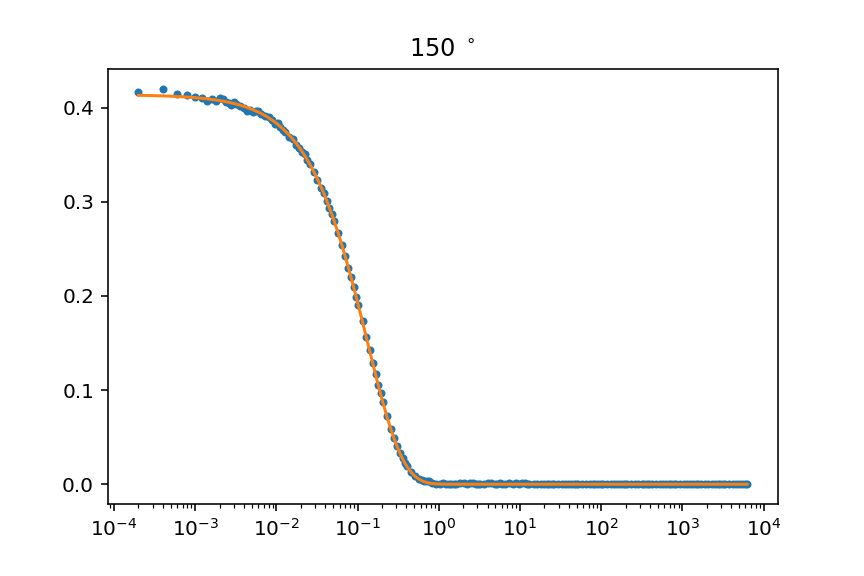
\includegraphics[width=\linewidth]{Plots/A/150.png}
\end{subfigure}

\caption{Autocorrelation Sample A: Angle between 80 and 150 degrees.}
\end{figure}
\newpage

\subsection{Autocorrelation B}
\label{autocorr B}
\begin{figure}[!h]
\centering

\begin{subfigure}{0.48\textwidth}
\includegraphics[width=\linewidth]{Plots/B/20.png}
\end{subfigure}
\begin{subfigure}[c]{0.48\linewidth}
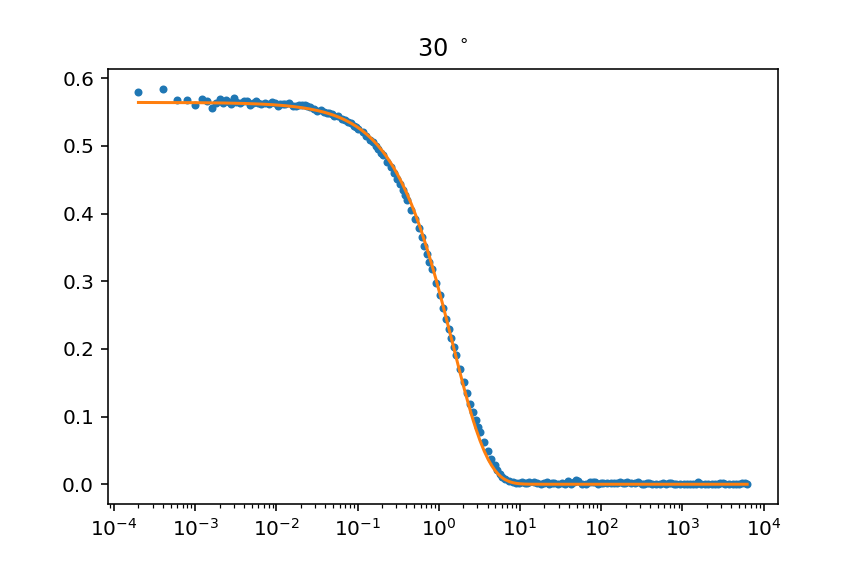
\includegraphics[width=\linewidth]{Plots/B/30.png}
\end{subfigure}

\medskip
\begin{subfigure}{0.48\textwidth}
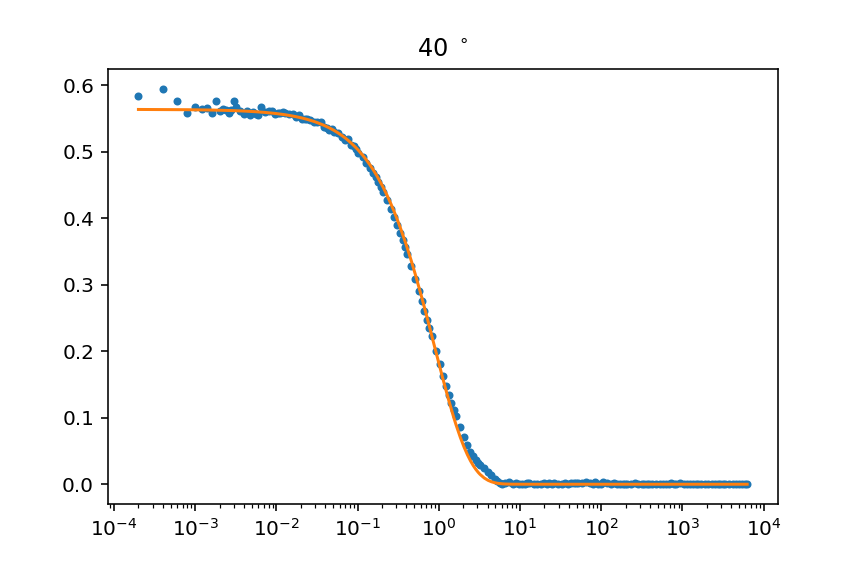
\includegraphics[width=\linewidth]{Plots/B/40.png}
\end{subfigure}
\begin{subfigure}[c]{0.48\linewidth}
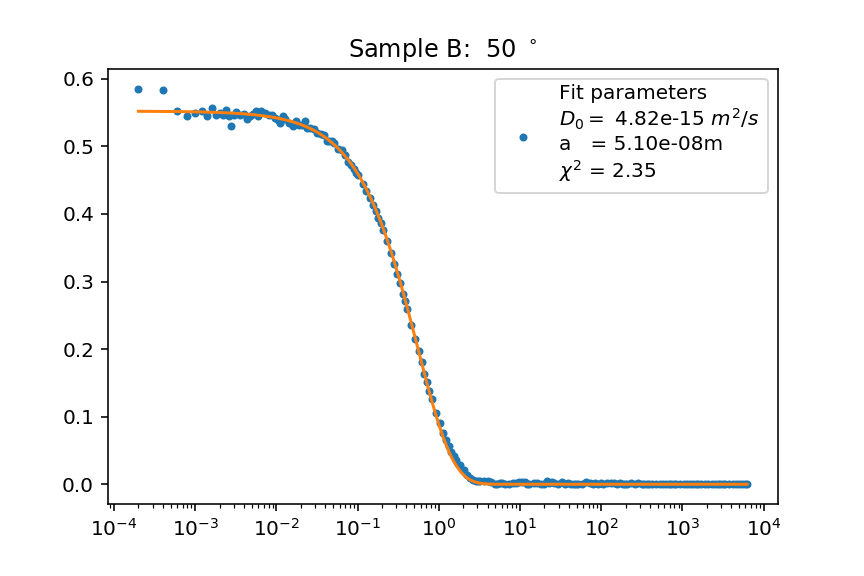
\includegraphics[width=\linewidth]{Plots/B/50.png}
\end{subfigure}

\medskip
\begin{subfigure}{0.48\textwidth}
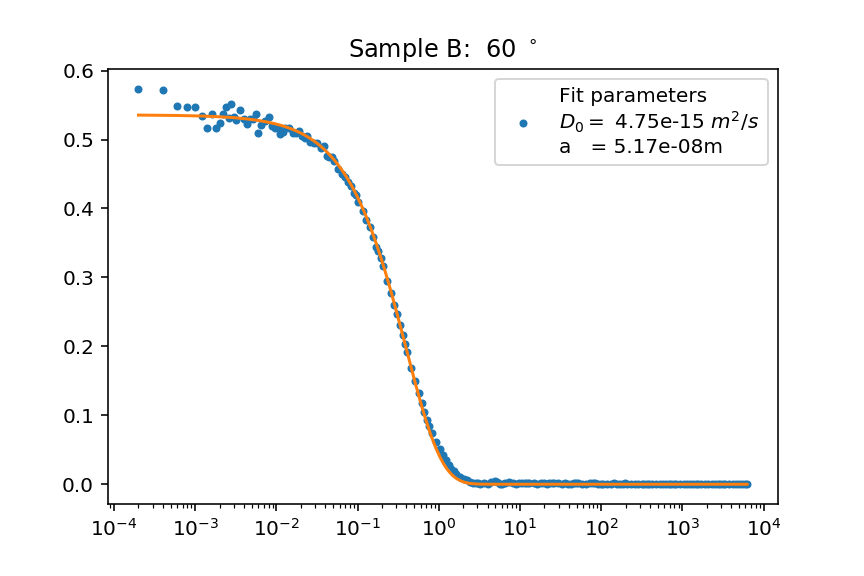
\includegraphics[width=\linewidth]{Plots/B/60.png}
\end{subfigure}
\begin{subfigure}[c]{0.48\linewidth}
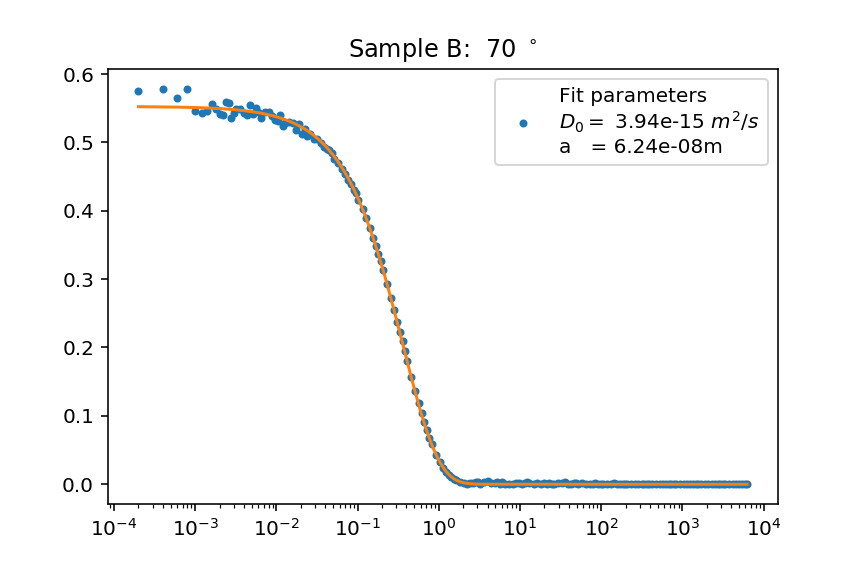
\includegraphics[width=\linewidth]{Plots/B/70.png}
\end{subfigure}

\caption{Autocorrelation Sample B: Angle between 20 and 70 degrees.}
\end{figure}
\newpage

\begin{figure}[!h]
\centering

\medskip
\begin{subfigure}{0.48\textwidth}
\includegraphics[width=\linewidth]{Plots/B/80.png}
\end{subfigure}
\begin{subfigure}[c]{0.48\linewidth}
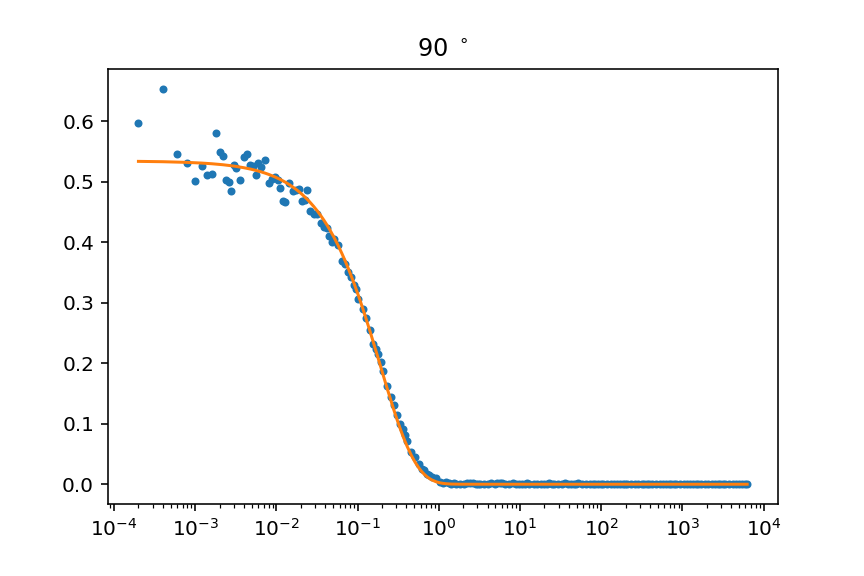
\includegraphics[width=\linewidth]{Plots/B/90.png}
\end{subfigure}

\medskip
\begin{subfigure}{0.48\textwidth}
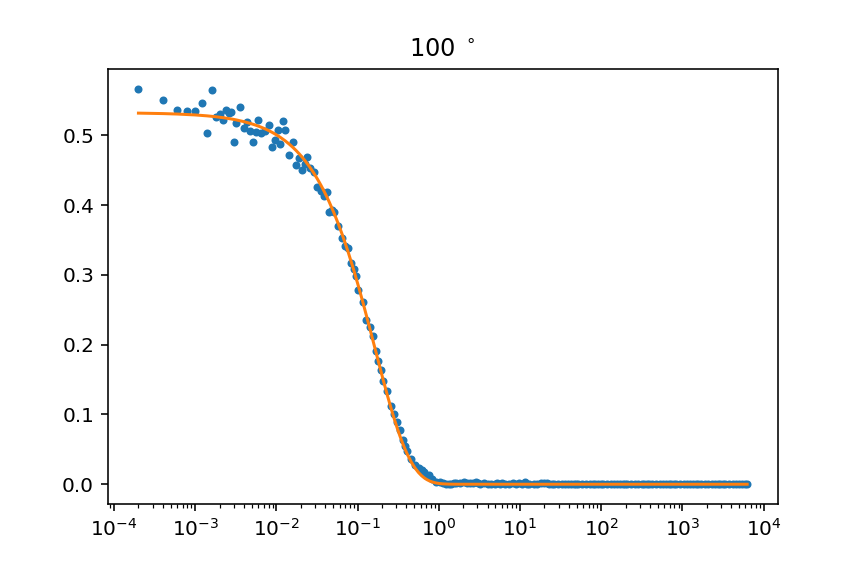
\includegraphics[width=\linewidth]{Plots/B/100.png}
\end{subfigure}
\begin{subfigure}[c]{0.48\linewidth}
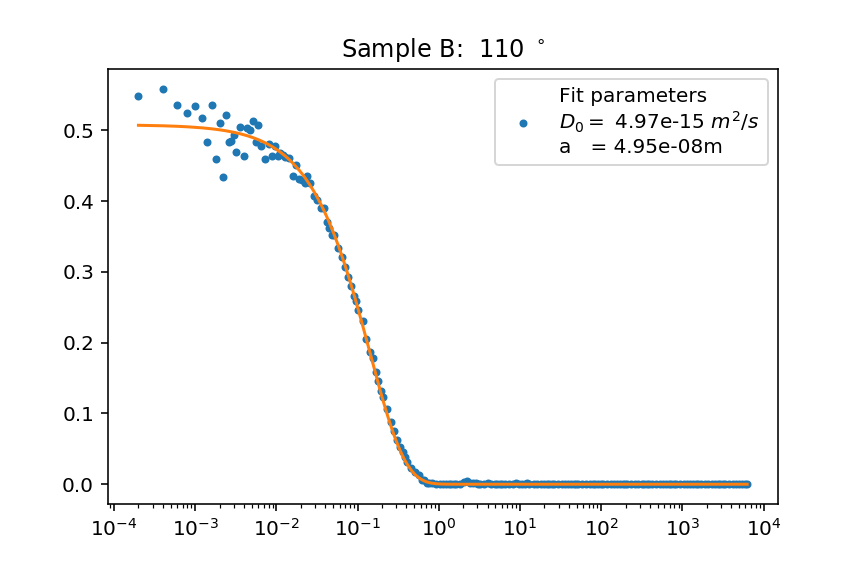
\includegraphics[width=\linewidth]{Plots/B/110.png}
\end{subfigure}

\medskip
\begin{subfigure}{0.48\textwidth}
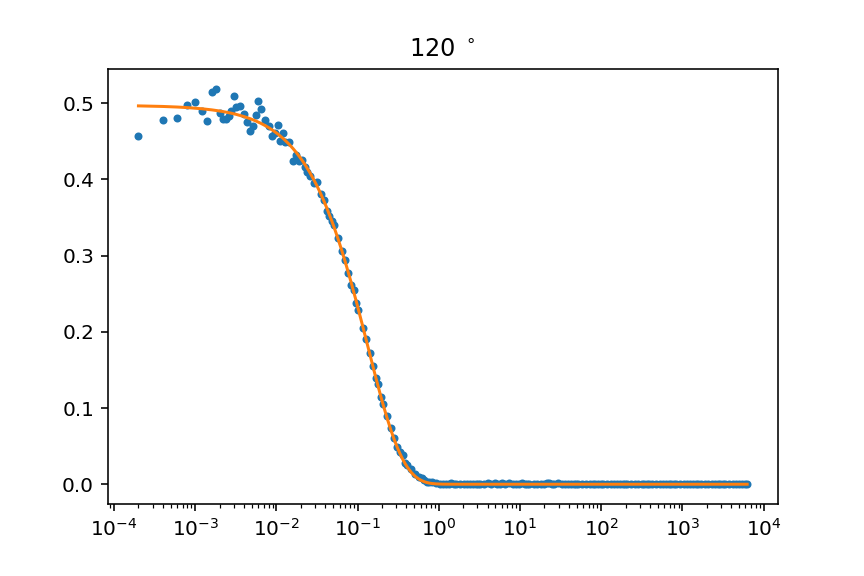
\includegraphics[width=\linewidth]{Plots/B/120.png}
\end{subfigure}
\begin{subfigure}[c]{0.48\linewidth}
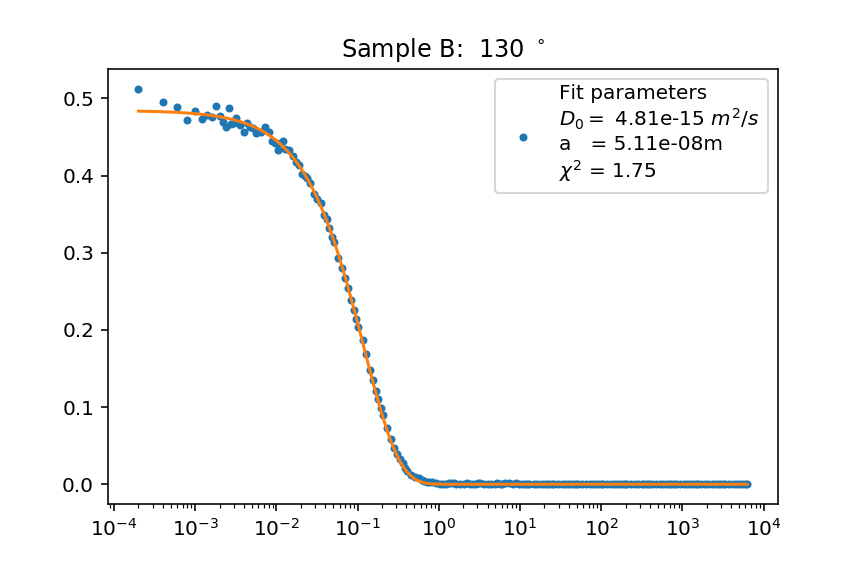
\includegraphics[width=\linewidth]{Plots/B/130.png}
\end{subfigure}

\medskip
\begin{subfigure}{0.48\textwidth}
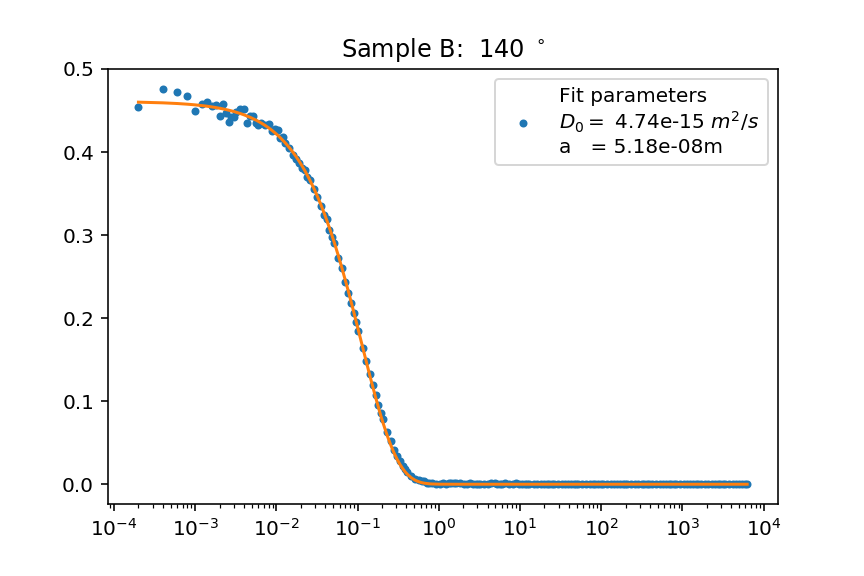
\includegraphics[width=\linewidth]{Plots/B/140.png}
\end{subfigure}
\begin{subfigure}[c]{0.48\linewidth}
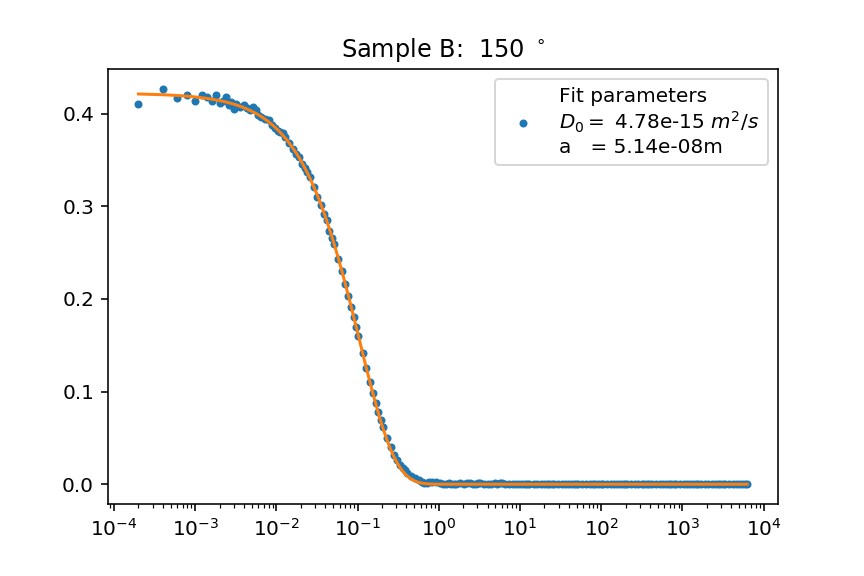
\includegraphics[width=\linewidth]{Plots/B/150.png}
\end{subfigure}

\caption{Autocorrelation Sample B: Angle between 80 and 150 degrees.}
\end{figure}


\newpage
\begin{thebibliography}{}

\bibitem{test} lulululululul

\end{thebibliography}
\end{document}

